\documentclass[a4paper, 11pt, notitlepage, english]{article}

\usepackage{babel, textcomp}
\usepackage[latin1]{inputenc}
\usepackage[T1]{fontenc, url}
\usepackage{amsmath, amssymb}
\usepackage{amsbsy, amsfonts}
\usepackage{graphicx, color, xcolor}
\usepackage{framed, parskip}
\usepackage{flafter, caption, multicol}
\usepackage{verbatim, listings, fancyvrb}


\usepackage{geometry}
\geometry{headheight=0.01mm}
\geometry{top=24mm, bottom=29mm, left=39mm, right=39mm}

\renewcommand{\arraystretch}{2}
\setlength{\tabcolsep}{10pt}
\makeatletter
\renewcommand*\env@matrix[1][*\c@MaxMatrixCols c]{%
  \hskip -\arraycolsep
  \let\@ifnextchar\new@ifnextchar
  \array{#1}}


\definecolor{javared}{rgb}{0.6,0,0} % for strings
\definecolor{javagreen}{rgb}{0.25,0.5,0.35} % comments
\definecolor{javapurple}{rgb}{0.5,0,0.35} % keywords
\definecolor{javadocblue}{rgb}{0.25,0.35,0.75} % javadoc

\lstset{language=python,
basicstyle=\ttfamily\scriptsize,
keywordstyle=\color{javapurple},%\bfseries,
stringstyle=\color{javared},
commentstyle=\color{javagreen},
morecomment=[s][\color{javadocblue}]{/**}{*/},
% numbers=left,
% numberstyle=\tiny\color{black},
stepnumber=2,
numbersep=10pt,
tabsize=4,
showspaces=false,
captionpos=b,
showstringspaces=false,
frame= single,
breaklines=true}

%
% Definering av egne kommandoer og miljøer
%
\newcommand{\dd}[1]{\ \text{d}#1}
\newcommand{\f}[2]{\frac{#1}{#2}} 
\newcommand{\beq}{\begin{equation*}}
\newcommand{\eeq}{\end{equation*}}
\newcommand{\bra}[1]{\langle #1|}
\newcommand{\ket}[1]{|#1 \rangle}
\newcommand{\braket}[2]{\langle #1 | #2 \rangle}
\newcommand{\braup}[1]{\langle #1 \left|\uparrow\rangle\right.}
\newcommand{\bradown}[1]{\langle #1 \left|\downarrow\rangle\right.}
\newcommand{\av}[1]{\left| #1 \right|}
\newcommand{\op}[1]{\hat{#1}}
\newcommand{\braopket}[3]{\langle #1 | {#2} | #3 \rangle}
\newcommand{\ketbra}[2]{\ket{#1}\bra{#2}}
\newcommand{\pp}[1]{\frac{\partial}{\partial #1}}
\newcommand{\ppn}[1]{\frac{\partial^2}{\partial #1^2}}
\newcommand{\up}{\left|\uparrow\rangle\right.}
\newcommand{\upup}{\left|\uparrow\uparrow\rangle\right.}
\newcommand{\down}{\left|\downarrow\rangle\right.}
\newcommand{\downdown}{\left|\downarrow\downarrow\rangle\right.}
\newcommand{\updown}{\left|\uparrow\downarrow\rangle\right.}
\newcommand{\downup}{\left|\downarrow\uparrow\rangle\right.}
\newcommand{\bupup}{\left.\langle\uparrow\uparrow\right|}
\newcommand{\bdowndown}{\left.\langle\downarrow\downarrow\right|}
\newcommand{\bupdown}{\left.\langle\uparrow\downarrow\right|}
\newcommand{\bdownup}{\left.\langle\downarrow\uparrow\right|}
\renewcommand{\d}{{\rm d}}
\newcommand{\Res}[2]{{\rm Res}(#1;#2)}
\newcommand{\To}{\quad\Rightarrow\quad}
\newcommand{\eps}{\epsilon}
\newcommand{\inner}[2]{\langle #1 , #2 \rangle}

\usepackage{caption}

%\DeclareCaptionLabelSeparator{colon}{. }
\renewcommand{\captionfont}{\sffamily}
\renewcommand{\captionlabelfont}{\bf\sffamily}
\setlength{\captionmargin}{40pt}

\newcommand{\bt}[1]{\boldsymbol{#1}}
\newcommand{\mat}[1]{\textsf{\textbf{#1}}}
\newcommand{\I}{\boldsymbol{\mathcal{I}}}
\newcommand{\p}{\partial}
%
% Navn og tittel
%
\author{Jonas van den Brink \\ \texttt{j.v.d.brink@fys.uio.no}}
\title{MAT-INF2360 \\ Project 1}

\usepackage{titling}
\usepackage{blindtext}
\setlength{\droptitle}{6em}


\begin{document}

\vspace {2cm}
\maketitle
\vspace {2 cm}
\section*{Abstract}
In this project, we will be looking at the discrete Fourier transform (DFT) and the 2-radix Cooley-Tukey fast Fourier transform (FFT) algorithm, which is a highly efficient algorithm for computing the DFT of a vector of length $2^n$.

We will look at the nature of the DFT, and how the FFT effectively cuts down the operations needed by exploiting symmetries in the transformation. 

In the first part of the project, we will write our own implementations of the FFT algorithm, as well as a simple implementation of the naive multiplication with the Fourier-matrix method of computing the DFT. We then compare these with the built-in \verb+fft+-function in NumPy.

In the second part of the project, we look at how the DFT can be used to do lossy compression of an audio-file by looking at the audio in frequency-space and eliminating certain ranges of frequencies.

\clearpage

\section*{The Discrete Fourier Transform}
Computing the DFT of a vector is a change of basis from the standard basis to Fourier basis: $\mathbb{R}^N \to \mathcal{F}_N$. Where the Fourier space is spanned from the pure digital tones of order $N$:
$$\mathcal{F}_N = \mbox{span}\big\{\bt{\phi}_n\big\}_{n=0}^{N-1}, \qquad \bt{\phi}_n = \frac{1}{\sqrt{N}}\big(1, e^{2\pi i n/N}, e^{2\pi i 2n/N}, \ldots, e^{2\pi i n(N-1)/N}.)$$
This change of basis is a linear transformation, so it can be written as a matrix multiplication:
$$\bt{y} = F_N \bt{x}.$$
Where $\bt{y}$ is the DFT of $\bt{x}$. The change-of-basis matrix $F_N$ is known as the $N$-point Fourier matrix, and it has the entries
$$(F_N)_{nk} = \frac{1}{\sqrt{N}}e^{-2\pi i n k/N},$$
where $0\leq n,k < N$.

The components of the DFT of $\bt{x}$ is thus given by
$$y_k = \frac{1}{\sqrt{N}}\sum_{n=0}^{N-1} x_n e^{-2\pi i nk /N}.$$

\subsection*{The 2-radix Cooley-Tukey FFT}
When computing the DFT of a $N$-length vector $\bt{x}$. If $\bt{x}$ is of even length, we can divide the computation of a single component into a sum over the even and odd terms of $\bt{x}$ as follows:
\begin{align*}
y_k &= \frac{1}{\sqrt{N}}\sum_{n=0}^{N-1} x_n e^{-2\pi i nk /N} \\
&= \frac{1}{\sqrt{N}}\bigg(\sum_{n=0}^{N/2-1} x_{2n} e^{-2\pi i 2nk /N} + \sum_{n=0}^{N/2-1} x_{2n+1} e^{-2\pi i (2n+1)k /N}\bigg)
\end{align*}
We now recognize that these partial sums look much like the original definition of the DFT. We make some adjustments
\begin{align*}
y_k &= \frac{1}{\sqrt{2}}\bigg(\frac{1}{\sqrt{N/2}}\sum_{n=0}^{N/2-1} x_{2n} e^{-2\pi i 2k /(N/2)} \\ 
&\qquad\qquad\qquad + e^{-2\pi i k/N} \frac{1}{\sqrt{N/2}}\sum_{n=0}^{N/2-1} x_{2n+1} e^{-2\pi i nk /(N/2)}\bigg).
\end{align*}
And so we see that we have reduced our original problem to computing two DFTs of length $N/2$. There is obviously no speed up so far, as two computations of $N/2$ times the $N$ components of $\bt{y}$ means we still have the complexity $\mathcal{O}(N^2)$.

However, we can now exploit some symmetries in the sub-problem DFTs. To see this, let us first introduce some short-hand notations for our sub-problem DFTs:
\begin{align*}
y_k^{(e)} &\equiv \frac{1}{\sqrt{N/2}}\sum_{n=0}^{N/2-1} x_{2n} e^{-2\pi i nk /(N/2)} \\
y_k^{(o)} &\equiv \frac{1}{\sqrt{N/2}}\sum_{n=0}^{N/2-1} x_{2n+1} e^{-2\pi i nk /(N/2)} \\
\end{align*}
We also introduce
$$D_k \equiv e^{-2\pi i k/N},$$
note that $D_k$ is simply a complex root of unity, and is often called a \emph{twiddle} factor in the FFT literature.

We have now shown that we can compute $y_k$ as
$$y_k = \frac{1}{\sqrt{2}}\bigg(y_k^{(e)} + D_k y_k^{(o)}\bigg),$$
for $k=0, \ldots, N-1$. Note that we have \emph{not} as of yet reduced the complexity of the problem at all. However, we are now ready to exploit the symmetries in the problem.

Note that the sub-DFTs only go from 0 to $N/2-1$. This means that we can compute $y_{k}^{(e)}$ and $y_{k}^{(o)}$ for $0\leq k < N/2$ using our favorite DFT algorithm, but what about the values for $N/2 \leq k < N$? This is where the symmetry comes in, notice that:
\begin{align}
y_{k + N/2}^{(e)}     
&= \frac{1}{\sqrt{N/2}}\sum_{n=0}^{N/2-1} x_{2n} e^{-2\pi i n(k+N/2) /(N/2)} \\
&= \frac{1}{\sqrt{N/2}}\sum_{n=0}^{N/2-1} x_{2n} e^{-2\pi i n}e^{-2\pi i nk /(N/2)}  \\ 
&= \frac{1}{\sqrt{N/2}}\sum_{n=0}^{N/2-1} x_{2n} e^{-2\pi i nk /(N/2)} \\[0.2cm]
&= y_{k}^{(e)}
\end{align}
And similarily we find
$$y_{k+N/2}^{(o)} = y_k^{(o)}.$$
What about the twiddle factor? We see that
$$D_{k+N/2} = e^{-2\pi i (k+N/2)/N} = e^{-\pi i}e^{-2\pi i k/N} = -D_{k},$$
So we see that we can drop as much as half of all our computations! As we 
only have to actually calculate $y_k^{(e)}$, $y_k^{(o)}$ and $D_k$ for $0\leq k < N/2$, we can then find $y_k$ for $0\leq k < N$ from:
\begin{align*}
y_k &= \frac{1}{\sqrt{2}}\bigg(y_k^{(e)} + D_k y_k^{(o)}\bigg), \\
y_{k+N/2} &= \frac{1}{\sqrt{2}}\bigg(y_k^{(e)} - D_k y_k^{(o)}\bigg).
\end{align*}
But the pay-off doesn't stop there, as long as $N/2$ is even, we can repeat the process for each of the sub-problems, meaning we get even more efficiency. In fact, as long as the original input is of length $N=2^n$ for some integer $n$, we see that each level reduces the number of computations needed, this effectively reduces the complexity to $\mathcal{O}(N\log N).$


\section*{Part 1 - Algorithms for computing the DFT}

In the first problem, we will be comparing four functions in Python for calculation the DFT of a real vector of $2^n$ samples. The functions we will be comparing are:
\begin{itemize}
    \item A naive matrix-multiplication implementation.
    \item A simple recursive implementation of the radix-2 Cooley-Tukey FFT algorithm.
    \item A vectorized version of the radix-2 Cooley-Tukey.
    \item The \verb+numpy.fft.fft+ function, which is a wrapper for the FFT from the FFTPACK library, which is a well-tested and highly efficient implementation of the FFT in Fortran.
\end{itemize}

\subsection*{(a) Implementations}
\textbf{Note:} The problem-text specified that we may assume that $\bt{x}$ is a column vector. While we will treat it as such mathematically, we will write our implementations as though it is a flat NumPy array. This is simply because it's more practical.


\subsubsection*{DFT by Matrix Multiplication}
Implementing the naive matrix-multiplication by the Fourier matrix is rather straight-forward using NumPy. The algorithm is as follows:
\begin{enumerate}
    \item Assemble the $N$-point Fourier matrix of the right size.
    \item Perform the matrix-vector multiplication: $F_n\bt{x}$.
\end{enumerate}
And the implementation in Python is almost as easy:
\begin{lstlisting}
def DFTImpl(x):
    '''
    Computes DFT of flat vector by multiplying with Fourier matrix.
    '''

    # Find the dimension of the input
    N = x.shape[0]

    # Assemble the N-point fourier-matrix
    n = arange(N)
    k = n.reshape((N,1))
    F_N = exp(-2j*pi*n*k/N)/sqrt(N)

    # Perform the matrix-multiplication
    return dot(F_N, x)
\end{lstlisting}
We now test the function by comparing the resulting DFT of some random samples to that of \verb+numpy.fft.fft+:
\begin{lstlisting}
x = random.random(1024)
print allclose(DFTImpl(x), fft.fft(x)/sqrt(1024))
\end{lstlisting}
Which returns \verb+True+. Note that we divide the result of \verb+numpy.fft.fft+ with $\sqrt{N}$ as the FFTPACK implementation uses a different normalization definition from what we are using.

\subsection*{DFT by a recursive FFT function}
We will now implement the 2-radix Cooley-Tukey FFT algorithm, which we described earlier. We will implement the algorithm recursively, calling the FFT-function for the sub-problems. This is not a very efficient solution, as it uses Python-stack recursions and a lot of memory for both function calls and temporary storage. However, the focus is on readability, not efficiency in this implementation.

The base case of our recursion will be when the length of our sub-vectors reaches some smallest size. We could let this length be $1$, and then simply return the input-vector back (the DFT of a vector of length 1 is the vector itself). Or we could let it reach some size where we use the matrix-multiplication function we just defined, i.e., call \verb+DFTImpl+. In this case, we will choose the last option. The complexity of the \verb+DFTImpl+ is $\mathcal{O}(N^2)$, so it scales poorly for large input, but as long as $N$ is small it is perfectly fine to use, so there is no issue with using it to solve our base case.

The algorithm is then as follows
\begin{enumerate}
    \item If the length of the input-vector is smaller than some cut-off, return the DFT by calling \verb+DFTImpl+.
    \item Recursively call the FFT-function for the even and odd terms of the input-vector.
    \item Assemble the twiddle-factor.
    \item Compute the two halves of the DFT, i.e., one for $0\leq k < N/2$ and one for $N/2\leq k < N$.
    \item Assemble the complete DFT by combining the two parts.
\end{enumerate}

Again the code is rather straight-forward

\begin{lstlisting}
def FFT_recursive(x):
    '''
    Computes the DFT of a flat vector recursively. 
    Uses DFTImpl for the base-case of N <= 32.
    '''
    N = x.shape[0]

    if N <= 32:
        return DFTImpl(x)

    ye = FFT_recursive(x[::2])
    yo = FFT_recursive(x[1::2])
    D = exp(-2j*pi*arange(N/2)/N)

    return concatenate([ye + D*yo, ye - D*yo])/sqrt(2)
\end{lstlisting}

Again we test this function against \verb+numpy.fft.fft+ for some random input, and confirm that is functions as intended.

\subsection*{A Vectorized FFT Function}
We will now write a more efficient version of the FFT algorithm. Although the recursion version is very easy to understand, it uses a lot of Python-calls and temporary storage of arrays in memory. Both of these are inefficient, instead we would like to use NumPy as much as possible. 

When using the recursive method, we are effectively making repeated recursive calls until we have an array of length 32 or less, and solving this sub-problem using \verb+DFTImpl+, only after we have calculated this first sub-DFT do we start returning upward, assembling larger parts of the total DFT as we go. It is easy to realize that we could in fact start of by doing \emph{all} of the lowest-order computations, and then all of the next-to-lowest assemblies, and continue upwards untill we have the complete DFT. This is the main idea of the vectorized FFT function.

The algorithm is as follows
\begin{enumerate}
    \item Reshape the flat NumPy array, which is originally $2^n$-long, into a $(32,2^{n-5})$ shaped array.
    \item Multiply the resulting matrix with the $32$-point Fourier matrix.
    \item Reassemble the total DFT by vertically stacking the matrix according to the FFT algorithm. Effectively halving the number of rows per repetition.
    \item When the matrix has been turned into a column-vector, collapse and return it.

\end{enumerate}

\begin{lstlisting}
def FFT_vectorized(x):
    # Find total number of elements
    N = x.shape[0]

    if N < 32:
        return DFTImpl(x)

    # Reshape flat vector into matrix and left-multiply by F32
    y = DFTImpl(x.reshape(32,-1))

    # Assemble total DFT layer by layer
    while y.shape[0] < N:
        ye = y[:, :y.shape[1]/2]
        yo = y[:, y.shape[1]/2:]
        D = exp(-1j*pi*arange(y.shape[0])/y.shape[0])[:, None]
        y = vstack([ye + D*yo, ye - D*yo])/sqrt(2)

    return y.ravel()
\end{lstlisting}

And again we confirm that it gives the same result as \verb+numpy.fft.fft+ for some random input.

\clearpage

\subsection*{(b) Timing the Functions}
We now time the functions by using the \verb+timeit+ module in Python. We use the audio-file \verb+castanets.wav+, and use the four functions to compute the DFT of the first $2^n$ samples of the first channel for $n=4,5,\ldots, 14$. The results are shown in table 1 and in figure 1 on the next two pages. The codes that was used to time the functions is as follows:
\begin{lstlisting}
from scitools import sound
from timeit import Timer

x = sound.read('castanets.wav')
x = x[::2]

setup = """
from __main__ import DFTImpl, FFT_recursive, FFT_vectorized, fft, x_sub
"""

ofile = open('times2.dat', 'a')

for n in range(18, 21):
    x_sub = x[:2**n]
    t1 = min(Timer("DFTImpl(x_sub)", setup=setup).repeat(2, 1))
    t2 = min(Timer("FFT_recursive(x_sub)", setup=setup).repeat(2, 1))
    t3 = min(Timer("FFT_vectorized(x_sub)", setup=setup).repeat(2, 1))
    t4 = min(Timer("fft.fft(x_sub)", setup=setup).repeat(2, 1))
    ofile.write("%i %.2e %.2e %.2e \n" % (n, t2, t3, t4))

ofile.close()    
\end{lstlisting}

We see that for $n=4$ and $n=5$, the results for the tree functions we have implemented are identical, the reason for this is of course that we are using the \verb+DFTImpl+-function for the base-case of 32 (i.e.\ n=5), so we are basicly using the same function. (I tried reducing the base case to return $x$ if $N=1$, in which case the recursive function bace slower than \verb+DFTImpl+). We see that the FFTPACK-function is already an order of magnitude faster than our functions.

As $n$ grows, we see that \verb+DFTImpl+ becomes slower very quickly, this should not be surprising as it has the complexity $\mathcal{O}(N^2)$. Increasing $n$ by one, means doubling $N$, which means the time used by the \verb+DFTImpl+-function should increase by a factor of ca 4, which we see is exactly what happens as $n$ increases.

Meanwhile, the complexity of all three FFT functions, is $\mathcal{O}(N\log N)$, meaning they scale a lot better. Not surprisingly we see that the recursive function is both the slowest, and scales the worst, of the three FFT functions. This is due to the massive amount of Python overhead that results from a large input. The vectorized function is faring rather well, but unsurprisingly it is beaten across the bort by a order of magnitude (or more) by the FFTPACK version.


\begin{table}
\centering
\begin{tabular}{c|c|c|c|c}
$n$ & \texttt{DFTImpl} & \texttt{FFT\_recursive} & \texttt{FFT\_vectorized} & \texttt{numpy.fft.fft} \\ \hline
4 & 5.60e-05 & 5.60e-05 & 5.60e-05 & 5.96e-06 \\ \hline
5 & 1.29e-04 & 1.30e-04 & 1.31e-04 & 6.91e-06 \\ \hline
6 & 4.11e-04 & 2.98e-04 & 2.03e-04 & 6.91e-06 \\ \hline
7 & 1.54e-03 & 6.36e-04 & 2.77e-04 & 7.87e-06 \\ \hline
8 & 6.04e-03 & 1.31e-03 & 3.75e-04 & 1.10e-05 \\ \hline
9 & 2.96e-02 & 2.68e-03 & 5.19e-04 & 1.98e-05 \\ \hline
10 & 1.24e-01 & 5.47e-03 & 7.65e-04 & 3.60e-05 \\ \hline
11 & 5.54e-01 & 1.11e-02 & 1.24e-03 & 6.89e-05 \\ \hline
12 & 2.11e+00 & 2.24e-02 & 2.27e-03 & 1.45e-04 \\ \hline
13 & 9.78e+00 & 4.54e-02 & 4.60e-03 & 3.73e-04 \\ \hline
14 & - & 9.09e-02 & 8.96e-03 & 7.83e-04 \\ \hline
\end{tabular}
\caption{Results of using \texttt{timeit.Timer} on the four functions with input of varying size. The times given are the min-values of a run of timer with repeat=3.}
\end{table}

\begin{figure}[thb]
\centering
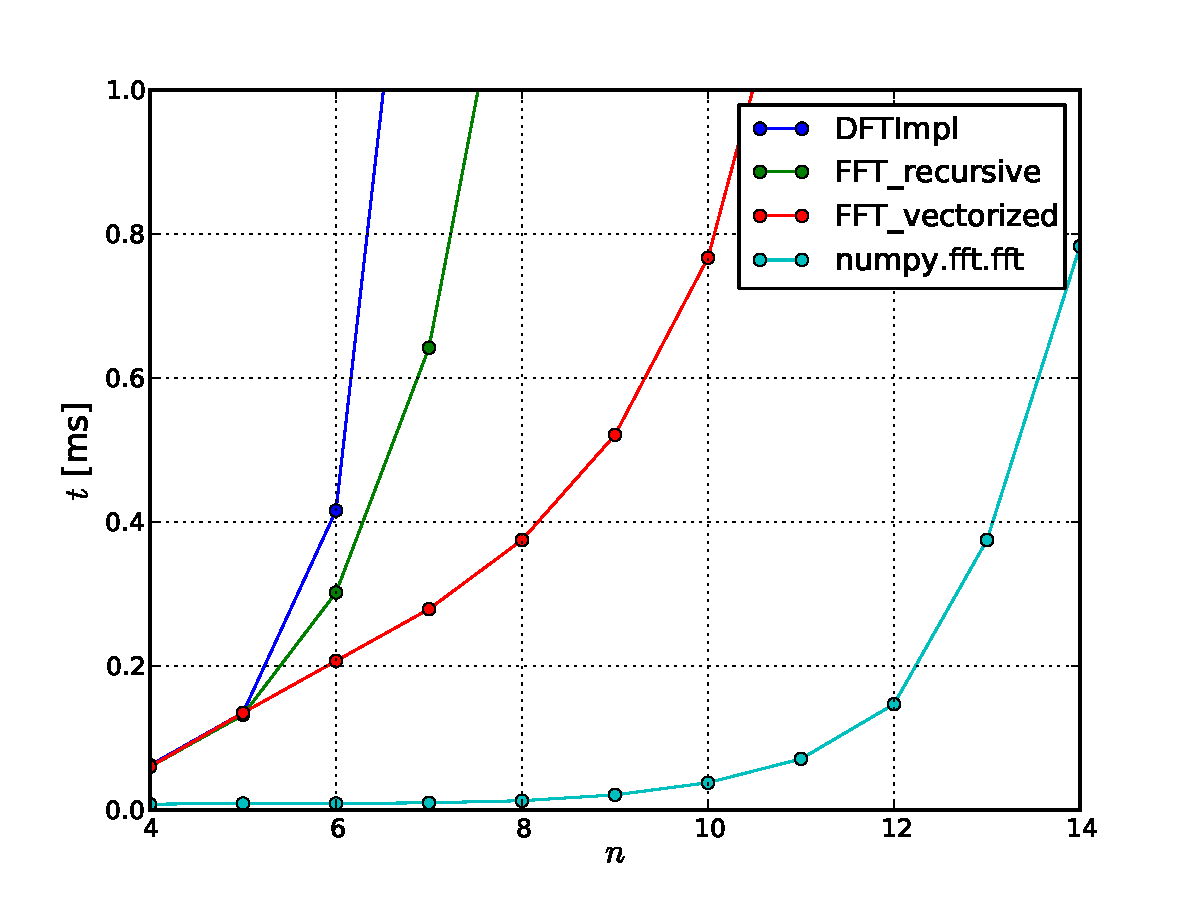
\includegraphics[width=0.75\textwidth]{times_a}
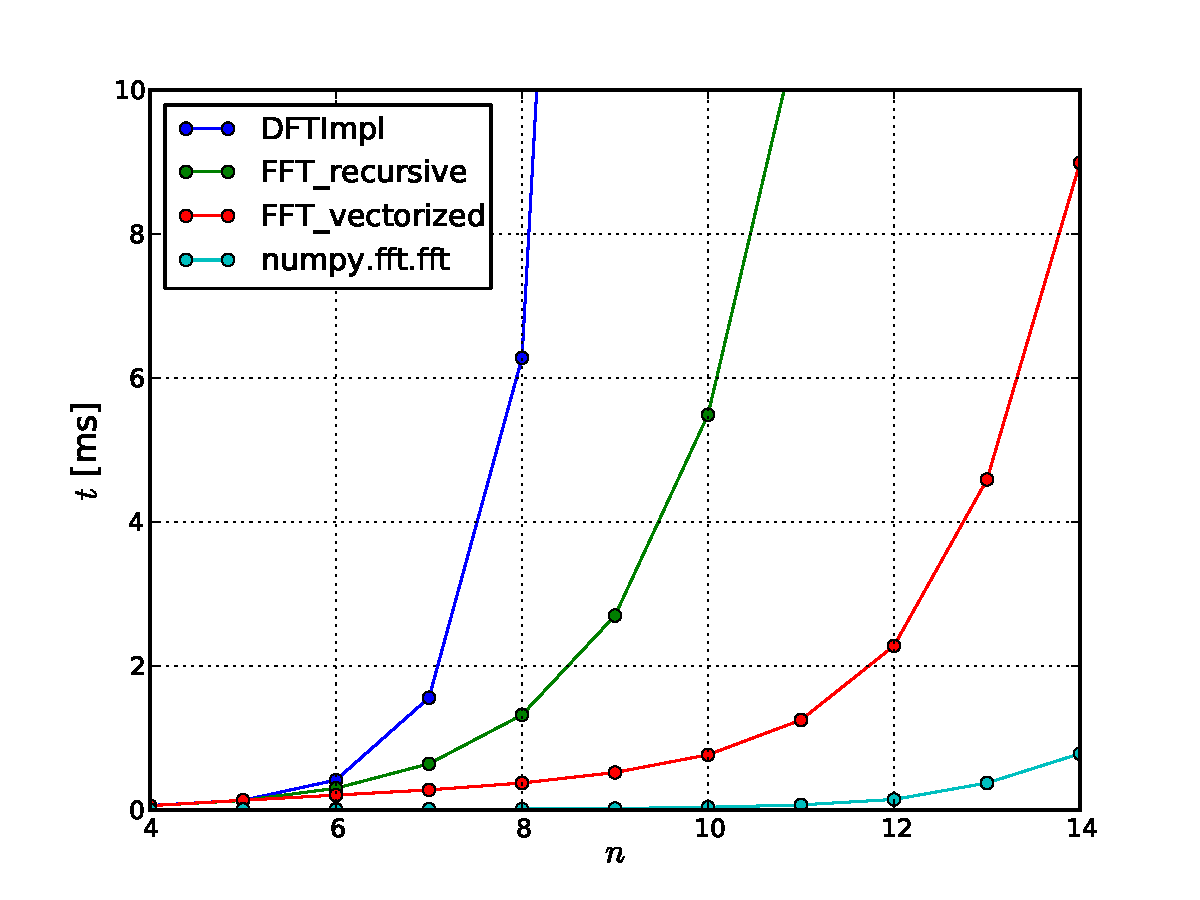
\includegraphics[width=0.75\textwidth]{times_b}
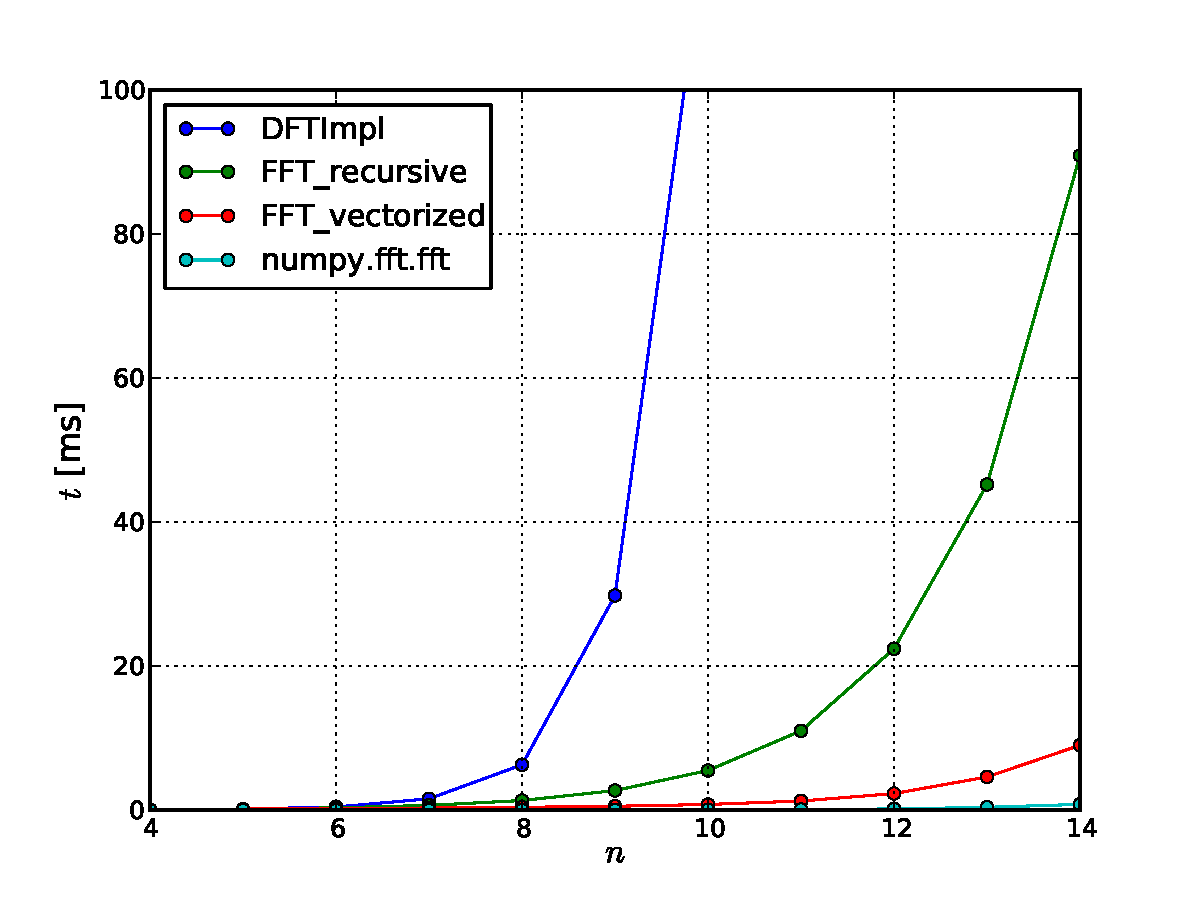
\includegraphics[width=0.75\textwidth]{times_c}
\caption{Times of the four DFT computations using the $2^n$ first samples of the audio-file.
\label{fig:contraction}}
\end{figure}

\clearpage

\subsection*{(c) DFT for Very Large Input}

We now time our FFT-functions for larger values of $n$. We disregard \verb+DFTImpl+ as it scales to poorly in the number of operations required, as well as the fact that it stores a matrix of size $N^2$ in memory, meaning it will max out our computers memory very quickly.

The sound file we are looking at has $2^{18} < 292570 < 2^{19}$ samples per channel. As we want to compare our FFT functions for $2^n$ for n=15,\ldots,22, we instead time them with random input generated from numpy.random.random. The following figure shows the results:

\begin{figure}[h]
\centering
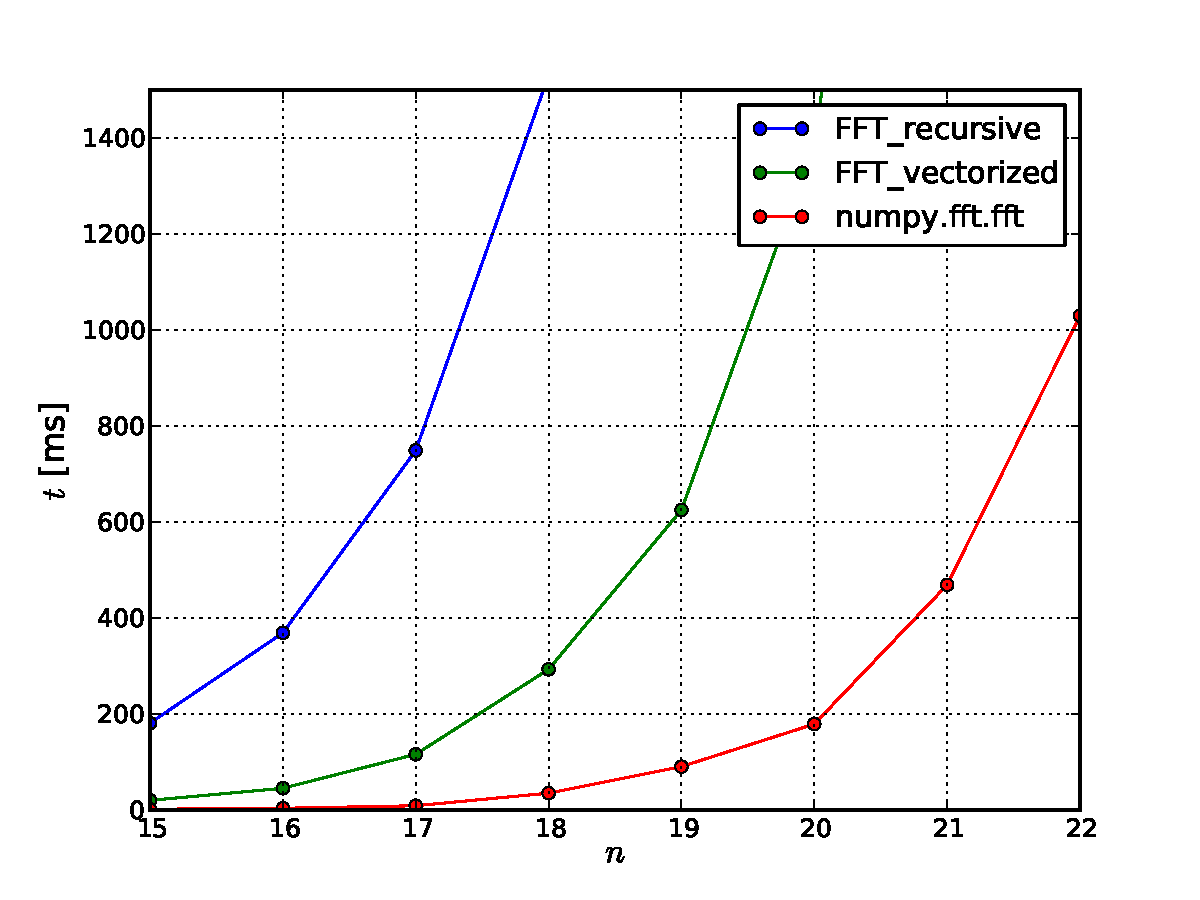
\includegraphics[width=0.8\textwidth]{times_d}
\caption{Times of the three FFT computations using random inputs of length $2^n$.}
\end{figure}

We see that while \verb+DFTImpl+ had to be disregarded already at $n=15$ due to both a massive running time, and limited memory. All three FFT functions can easily handle inputs of as much as $2^{22}$ (and even higher), due to a superior algorithm. We see that while the three functions all scale as $\mathcal{O}(N\log N)$, the FFTPACK-function is clearly superior at all times, although no longer by over an order of magnitude.

The FFTPACK-function is superior due to beeing a Fortran implementation that is highly optimized. We cannot possibly hope to achieve the same speed in Python without using wrappers like those the \verb+numpy.fft+-module provides.

\clearpage

\section*{Part 2 - Lossy Compression of Sound through DFT}
We will now use the DFT of an audio signal to do lossy compression of it. 

\subsection*{(a) An Inverse Discrete Fourier Algorithm (IDFT)}
As we described earlier, the DFT of a vector $\bt{x}$, is simply a change of basis:
$$\bt{y} = F_N \bt{x}.$$
The \emph{inverse} DFT, is simply the reverse change of basis, i.e.,
$$\bt{x} = (F_N)^{-1} \bt{y}.$$
Finding the inverse Fourier matrix is rather simple, as it is unitary. Meaning we find the inverse matrix by taking the conjugate transpose of $F_N$, so we have
$$x_k = \frac{1}{\sqrt{N}}\sum_{n=0}^{N-1}y_n e^{2\pi i n k/N}.$$

We now implment an inverse version of our vectorized FFT function, meaning we also have to make a \verb+IDFTImpl+-function for the base-case.
\begin{lstlisting}
def IDFTImpl(y):
    '''
    Computes the IDFT of vector y through matrix-multiplication
    '''
    N = y.shape[0]

    # Assemple the N-point inverse fourier-matrix
    n = arange(N)
    k = n.reshape((N,1))
    F_N = exp(2j*pi*n*k/N)/sqrt(N)

    return dot(F_N, y)


def IFFT_vectorized(y):
    '''
    Vectorized impl. of the IFFT
    '''
    # Find total number of elements
    N = y.shape[0]

    if N < 32:
       return IDFTImpl(y)

    # Reshape vector into lower-order subproblem and solve it
    x = IDFTImpl(y.reshape(32,-1))

    # Assemble total IDFT layer by layer
    while x.shape[0] < N:
        xe = x[:, :x.shape[1]/2]
        xo = x[:, x.shape[1]/2:]
        D = exp(1j*pi*arange(x.shape[0])/x.shape[0])[:, None]
        x = vstack([xe + D*xo, xe - D*xo])/sqrt(2)

    return x.ravel()
\end{lstlisting}

\clearpage

As a test, we try first calculating the DFT of some random data, and then computing the IDFT, and checking if we end up at the original data:
\begin{lstlisting}
x = random.random(1024)
y = FFT_vectorized(x)
print allclose(x, IFFT_vectorized(y))    
\end{lstlisting}
\vspace{-0.3cm}
And we see that everything functions as intended.

\subsection*{(b) Plotting the DFT-coefficients for an Audio Signal}

We now extract the first $2^{17}$ samples from the audio signal in the file \verb+castanets.wav+. We compute the DFT of the samples and plot the resulting coefficients. 

\begin{lstlisting}
from scitools.sound import read

# Extract the first 2**17 samples from the first channel
x = read('castanets.wav')
x = x[::2]
x = x[:2**17]

# Calculate the DFT coefficients
y = FFT_vectorized(x)

# Plot
plot(abs(y)/(max(abs(y))))
axis([0, N, 0, 1.1])
xlabel(r'DFT index', fontsize=16)
ylabel(r'Magnitude of DFT coefficients [scaled]', fontsize=16)
grid()
savefig('DFT_coeffs_index.pdf')
show()
\end{lstlisting}

Figure 3 and 4 on the next page show the resulting DFT coefficients. In figur 3 we plot the magnitude of all the DFT coefficients against their indices. We see that the plot is mirrored around $N/2$ as expected due to folding.

To better understand how these coefficients correspond to frequencies, we plot the first half of the coefficients against their corresponding frequencies, this is shown in figure 4. From this figure we read of the frequency distribution of the samples from the audio signal.



\begin{figure}[p]
\centering
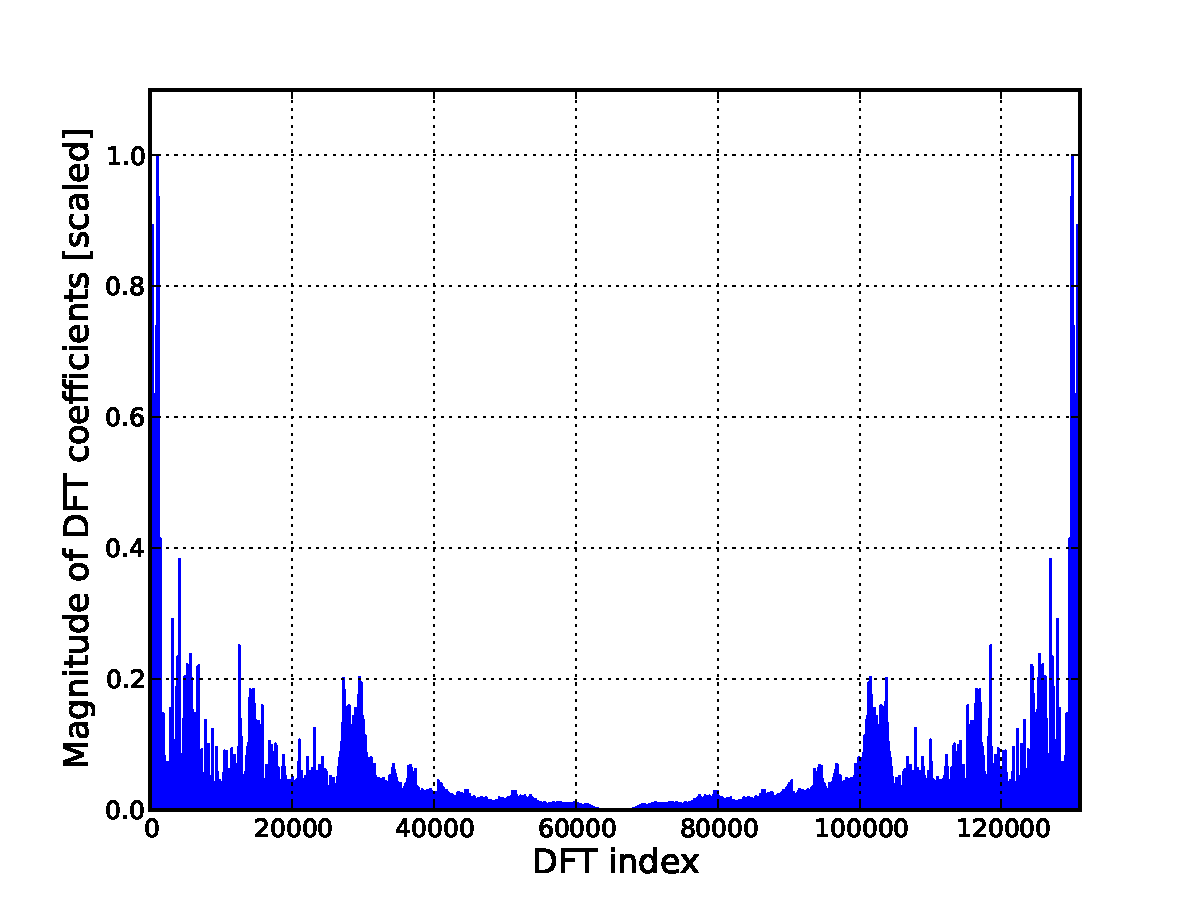
\includegraphics[width=\textwidth]{DFT_coeffs_index}
\caption{The magnitude of the DFT coefficients plotted against their index.}
\end{figure}

\begin{figure}[p]
\centering
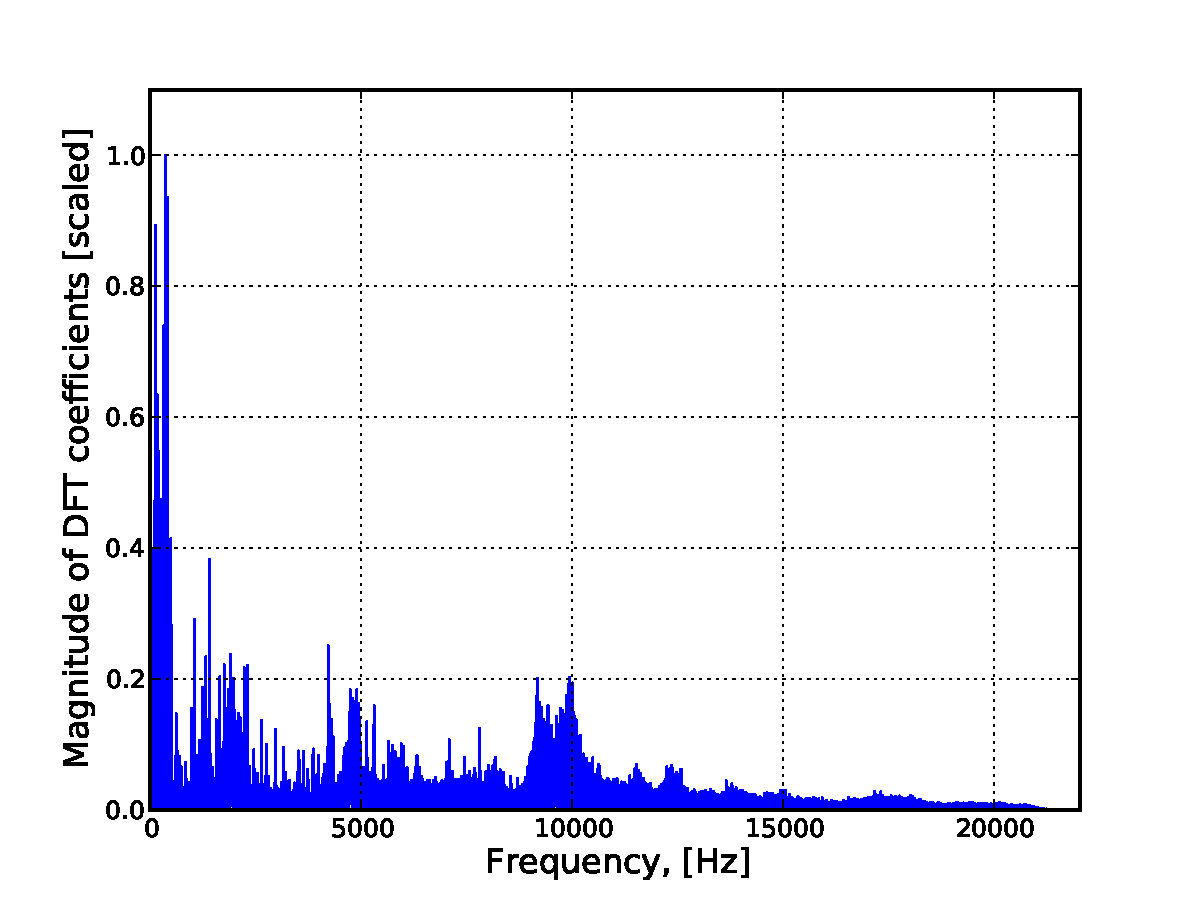
\includegraphics[width=\textwidth]{DFT_coeffs}
\caption{The magnitude of the DFT coefficients plotted against the corresponding frequencies they represent, the folding is not shown (i.e., the coefficients for indices over $N/2$ are not shown).}
\end{figure}

\clearpage

\subsection*{(c) DFT-coefficients and Frequency}

We have the following two observations:

\begin{itemize}
    \item \textbf{(Connection between DFT index and frequency)} \\
    Assume that we take N samples of a sound with sampling frequency $f_s$. Then DFT index $n$ corresponds the frequency $\nu = nf_s/N$.
    \item \textbf{(DFT indices for high and low frequencies)} \\
    When $\bt{y}$ is the DFT of $\bt{x}$, the low frequencies in $\bt{x}$ correspond to the indices in $\bt{y}$ near $0$ and $N$. The high frequencies in $\bt{x}$ correspond to the indices in $\bt{y}$ near $N/2$.
\end{itemize}

The second observation describes the folding or mirroring we see in the plot of the DFT-coefficients against their indices.

We now want to see what indices correspond to frequencies above 5000 Hz. We have
$$\nu = nf_s/N > 5000 \mbox{ Hz},$$
with $N=2^17$ and $f_s = 44100 \mbox{ Hz}$, giving
$$n < 14861.$$
And of course, due to the mirroring, we also disregard
$$N/2 < n < N-14861.$$
So the DFT-indices corresponding to frequencies over 5000 Hz are:
$$14861 < n < 116211.$$

\subsection*{(d) Removing frequencies}

We now explicitly set the DFT coefficients in the range we just found to 0.
\begin{lstlisting}
N = len(y)-1
fs = 44100.
max_freq = 5000

min_index = ceil(max_freq*N/fs)
max_index = N-min_index

y[min_index:max_index] = 0    
\end{lstlisting}

We can again plot the DFT-coefficients against their indices and against corresponding frequencies, giving the plots show on the next page.


\begin{figure}[p]
\centering
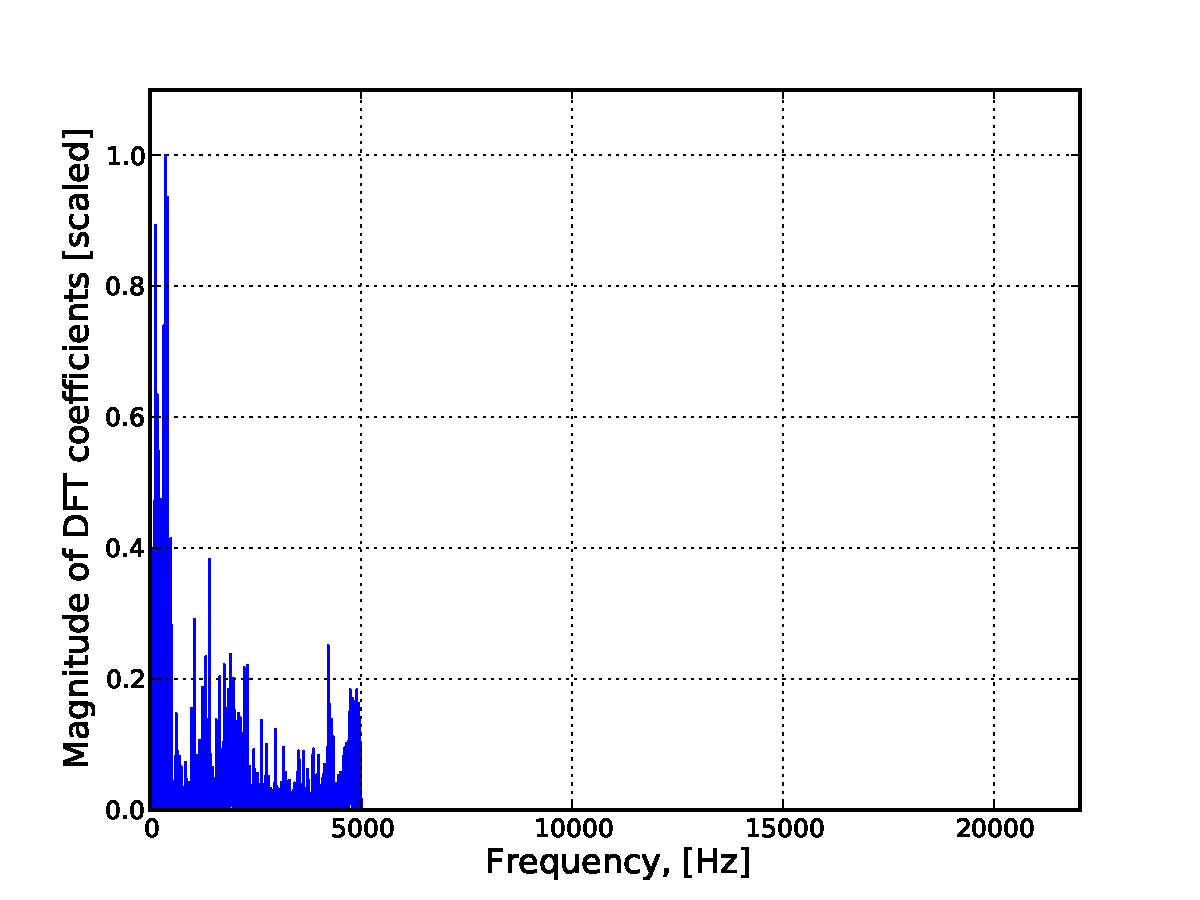
\includegraphics[width=\textwidth]{trunc}
\caption{The magnitude of the DFT coefficients plotted against their index, when indices corresponding to $\nu > 5000$ Hz have been removed.}
\end{figure}

\begin{figure}[p]
\centering
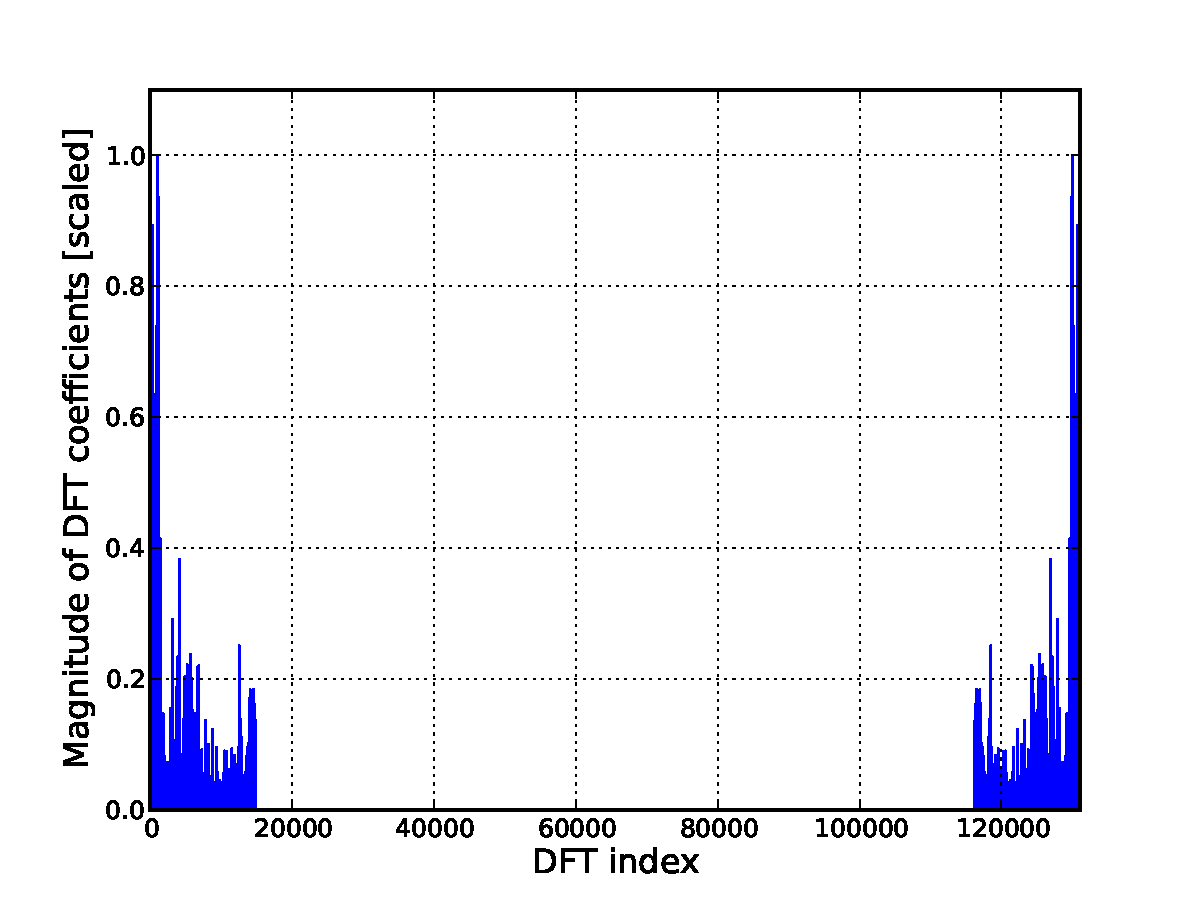
\includegraphics[width=\textwidth]{trunc2}
\caption{The magnitude of the DFT coefficients plotted against the corresponding frequencies they represent, after coefficients corresponding to $\nu > 5000$ Hz have been removed.}
\end{figure}

We now compute the IDFT of the remaining coefficients, and play the resulting sound.
\begin{lstlisting}
x = IFFT_vectorized(y)
x = real(x)
write(x, 'max_f=5000.wav')
play('max_f=5000.wav')        
\end{lstlisting}
    
When listening to the resulting audio file, we clearly recognize the earlier piece, and a bit of side-by-side comparision is requried to spot the details.

First of, we notice that the file with truncated frequencies is a generally more bassy and lower. This isn't surprising, as we have removed higher frequencies, which means we have removed the higher tones. 

At first, we might suspect the guitar to sound unaltered, but careful listening reveals that we seem to have lost the higher harmonics of the guitar playing, making it more flat. Harmonics are integer multiplices of the ground note, meaning removing higher frequencies will often also remove the higher harmonics of many instruments.

We also hear that the clicking sounds sound duller with the truncated frequencies, this may also be due to the higher harmonics being removed, although it is harder to say for sure here.

All in all, the conclusion is that there is quite a lot of difference between the originial and the truncated pieces. The original has more detail and generally sounds nicer. However, one has to remember that we have truncated 100\% of all frequencies above 5000 Hz, effectively compressing our DFT-coefficients by more than 75\%. This is a really impressive amount of compression! Also, we haven't really done any decent attempt at figuring out what frequencies to truncate, we simply threw \emph{all} frequencies above 5000 out, all of them. That is a brutal way to do compression of an audio-signal! All in all, I have to say I am impressed by how similar the audio sounds, considering our rough treatment of the raw data.

\subsubsection*{Truncating all $\nu > 3000$ Hz.}

Let us try truncating all frequencies above 3000 Hz. Right away we notice that the change in sound is a lot more pronounced. It generally has become even lower, lacking any higher notes at all. The sound is dull and pretty aweful to listen to.

\subsubsection*{(e) Truncating low frequencies ($\nu < 4000$ Hz).}

We now truncate all DFT-coefficients that correspond to frequencies lower than 4000 Hz.
\begin{lstlisting}
y[:min_index] = 0
y[max_index:] = 0    
\end{lstlisting}

When playing the audio, we hear that only a few high notes remain, all the bassy tones are completely gone (unsurprising). We can only hear the highest harmonics of the guitar and the clicking. The sound is pretty horrible to listen to.



\end{document}